\documentclass[8pt]{beamer}

\newif\ifplacelogo % create a new conditional
\placelogotrue % set it to true

\usetheme{Warsaw}
\usecolortheme{rose}
\usepackage{multicol}
\usepackage{epstopdf}
\usepackage[italic]{hepnames}
\usepackage{tikz}
\usepackage{listings}
\usepackage{times}
\usepackage{amsmath}
\usepackage{verbatim}
\usepackage{hyperref}
\usepackage{bbding}
\usepackage{gensymb}
\usepackage{upgreek}
\lstset{breakatwhitespace,
language=C++,
columns=fullflexible,
keepspaces,
breaklines,
tabsize=3, 
showstringspaces=false,
extendedchars=true}

% TikZ includes!!!
\usepackage{tikz}
\usetikzlibrary{backgrounds}
\usetikzlibrary{calc}
\tikzstyle{every picture}+=[remember picture]
\input{/home/oviazlo/Desktop/beamerPresentations/myReports/latexHelpScripts/tikzGrid.tex}


\begin{document}

% custom colors
\definecolor{olive}{rgb}{0.3, 0.4, .1}
\definecolor{fore}{RGB}{249,242,215}
\definecolor{back}{RGB}{51,51,51}
\definecolor{title}{RGB}{255,0,90}
\definecolor{dgreen}{rgb}{0.,0.6,0.}
\definecolor{gold}{rgb}{1.,0.84,0.}
\definecolor{JungleGreen}{cmyk}{0.99,0,0.52,0}
\definecolor{BlueGreen}{cmyk}{0.85,0,0.33,0}
\definecolor{RawSienna}{cmyk}{0,0.72,1,0.45}
\definecolor{Magenta}{cmyk}{0,1,0,0}

\definecolor{PixelColor}{RGB}{207,232,139}
\definecolor{SCTColor}{RGB}{167,166,255}
\definecolor{TRTColor}{RGB}{250,224,140}
\definecolor{grayColor}{RGB}{153,153,153}

\newcommand{\yRefPosOne}{0.0}
\newcommand{\xRefPosOne}{0.0}
\newcommand{\yRefPosTwo}{0.0}
\newcommand{\xRefPosTwo}{0.0}
\newcommand{\yRefIncrementOne}{0.0}
\newcommand{\xRefIncrementOne}{0.0}
\newcommand{\yRefIncrementTwo}{0.0}
\newcommand{\xRefIncrementTwo}{0.0}

\graphicspath{ {/home/oviazlo/Desktop/beamerPresentations/FCCee/pictures/CALOR2018/} }


\DeclareGraphicsExtensions{.eps, .pdf, .png}

\newcommand{\myBox}[2][pink] {
    \noindent\colorbox{#1}{
	\textbf{#2}
    }\par
}

% For nice block (provided by Oleh)
\tikzstyle{myBox} = [draw=red, fill=blue!1, very thick,
    rectangle, rounded corners, inner sep=5pt, inner ysep=9pt]
    
\tikzstyle{PixelBox} = [draw=PixelColor, fill=blue!1, very thick,
    rectangle, rounded corners, inner sep=5pt, inner ysep=9pt]
\tikzstyle{SCTBox} = [draw=SCTColor, fill=blue!1, very thick,
    rectangle, rounded corners, inner sep=5pt, inner ysep=9pt]
\tikzstyle{TRTBox} = [draw=TRTColor, fill=blue!1, very thick,
    rectangle, rounded corners, inner sep=5pt, inner ysep=9pt]

% poster advertisement
\newcommand{\myCenterBox}[2][pink] {
   {\centering
    \noindent\colorbox{#1}{
	\textbf{#2}
    }\par
  }
}

\newcommand{\mySmallCenterBox}[2][pink] {
   {\centering
    \noindent\colorbox{#1}{
	\textbf{{\small #2}}
    }\par
  }
}

\newcommand{\myVerySmallCenterBox}[2][pink] {
   {\centering
    \noindent\colorbox{#1}{
	\textbf{{\scriptsize #2}}
    }\par
  }
}

\newcommand{\backupbegin}{
   \newcounter{finalframe}
   \setcounter{finalframe}{\value{framenumber}}
}
\newcommand{\backupend}{
   \setcounter{framenumber}{\value{finalframe}}
}

\newcommand{\myNode}{\tikz[baseline,inner sep=1pt] \node[anchor=base]}

\tikzstyle{fancytitle} =[fill=white!15, text=black]

\definecolor{light-gray}{gray}{0.95}
% poster advertisement


\title[Calorimetry performance with CLD \hspace{14.0em}\insertframenumber/
\inserttotalframenumber]{ Calorimetry performance with CLD }


	\author[Oleksandr Viazlo]{Oleksandr Viazlo\\ 
	{\small on behalf of the CLICdp and FCC-ee collaborations}
	}
	\institute{\small CERN\\} 
	
       
	\date{22 May 2018}

% 	\logo{ \ifplacelogo \includegraphics[height=1.8cm]{./ID_week2/lund_uni-logo_s.pdf} \hspace{0.4cm} \fi}

	
%    	\frame{\titlepage}

   	

\placelogofalse

%*****************************************************************************
% \bgroup
% \setbeamercolor{background canvas}{bg=white}
\begin{frame}{}

    \begin{tikzpicture}[overlay]

    %% HELPER draw advanced helping grid with axises:
%     \draw (0,-5) to[grid with coordinates] (11,3);

    \node[right] (textNode) at (4,0) {
      { \large \bf Pion ID efficiency}
    };
    


    \end{tikzpicture}

\end{frame}
% \egroup
%*****************************************************************************
%*****************************************************************************
\begin{frame}{\large \large Single particle identification efficiency}
\renewcommand{\yRefPosOne}{-0.9}
\renewcommand{\xRefPosOne}{4.2}
\renewcommand{\xRefIncrementOne}{7.5}
\begin{tikzpicture}[overlay]

 \node[inner sep=0pt] (tmp) at (\xRefPosOne-1.7,\yRefPosOne-0.6)
%   {\includegraphics[width=6cm]{singleParticleEff/CLD_muon_eff.pdf}};
  {\includegraphics[width=6cm]{may21_muons_eff.pdf}};
  
 \node[inner sep=0pt] (tmp) at (\xRefPosOne+4.5,\yRefPosOne-0.6)
%   {\includegraphics[width=6cm]{singleParticleEff/CLD_pion_eff.pdf}};
  {\includegraphics[width=6cm]{may21_pions_eff.pdf}};


 \node  at (\xRefPosOne+1,\yRefPosOne+3.3) (box){%
    \begin{minipage}{1.1\textwidth}
  \begin{itemize}

   \item Efficiency = fraction of matched reconstructed particles out of the simulated MC particles:
      \begin{itemize}
       \item reconstructed particle of the same type as simulated MC particle
       \item angular matching: $\Delta\theta <$ 1 mrad and $\Delta\phi <$ 2 mrad
       \item energy matching:\\
       - charged particles: $|p_T^{truth} - p_T^{PFO}| < 5\%$ $p_T^{truth} $ \\
       - photons: $\Delta$$E < 5\times\sigma$(ECal) $\approx 0.75\times \sqrt{E}$
      \end{itemize}
    \end{itemize}
    \end{minipage}
  };

  \node [TRTBox]  at (\xRefPosOne+4.8,\yRefPosOne+2.7) (box){%
  \begin{minipage}{0.4\textwidth}
   Sample: single particles with flat cos($\theta$) distribution and fixed energy
  \end{minipage}
  };


  
         \node  at (\xRefPosOne-3.1,\yRefPosOne+1.75) (box){%
    \myCenterBox{\small Muons}
    };     

       \node  at (\xRefPosOne+3,\yRefPosOne+1.75) (box){%
    \myCenterBox{\small Pions}
    };     

 \node[inner sep=0pt] (tmp) at (\xRefPosOne-0.1,\yRefPosOne+1.75)
  {\tiny WORK IN PROGRESS};
 
 \node[inner sep=0pt] (tmp) at (\xRefPosOne+6.1,\yRefPosOne+1.75)
  {\tiny WORK IN PROGRESS};
    
 \node  at (\xRefPosOne+1,\yRefPosOne-3.5) (box){%
    \begin{minipage}{\textwidth}
      \begin{itemize}
        \item $>$99$\%$ muon efficiency and 93-96$\%$ pion efficiency for E$>$10 GeV
        \item Inefficiency at high energies with CLD is caused by a larger rate of pions being mis-reconstructed as muons 
%         $\to$ optimization of muon requirements are needed
      \end{itemize}
    \end{minipage}
  };
 
 \end{tikzpicture}
\end{frame}
%*****************************************************************************
%*****************************************************************************
\begin{frame}{\large \large Pion identification efficiency (CLD)}
\renewcommand{\yRefPosOne}{-0.5}
\renewcommand{\xRefPosOne}{4.2}
\renewcommand{\xRefIncrementOne}{7.5}
\begin{tikzpicture}[overlay]

 \node[inner sep=0pt] (tmp) at (\xRefPosOne-1.7,\yRefPosOne-0.6)
  {\includegraphics[width=6cm]{../plots_FCCweek_workshop/singleParticleEff/pion_eff_vs_theta_E20.pdf}}; 
  
 \node[inner sep=0pt] (tmp) at (\xRefPosOne+4.5,\yRefPosOne-0.6)
  {\includegraphics[width=6cm]{../plots_FCCweek_workshop/singleParticleEff/pion_eff_vs_theta_E100.pdf}};


 \node  at (\xRefPosOne+1,\yRefPosOne+2.9) (box){%
    \begin{minipage}{1.1\textwidth}
  \begin{itemize}

   \item Pion ID efficiency and inefficiency as function of cos($\theta$)
    \end{itemize}
    \end{minipage}
  };


 \node  at (\xRefPosOne+1,\yRefPosOne-3.5) (box){%
    \begin{minipage}{\textwidth}
      \begin{itemize}
        \item High momentum pions more often are misreconstructed as muons in barrel
      \end{itemize}
    \end{minipage}
  };
   
       \node  at (\xRefPosOne-2.65,\yRefPosOne+1.75) (box){%
    \myCenterBox{\small 20 GeV pions}
    };     

       \node  at (\xRefPosOne+3.6,\yRefPosOne+1.75) (box){%
    \myCenterBox{\small 100 GeV pions}
    };     

%  \node[inner sep=0pt] (tmp) at (\xRefPosOne-0.1,\yRefPosOne+1.75)
%   {\tiny WORK IN PROGRESS};
%  
%  \node[inner sep=0pt] (tmp) at (\xRefPosOne+6.1,\yRefPosOne+1.75)
%   {\tiny WORK IN PROGRESS};
    
 \end{tikzpicture}
\end{frame}
%*****************************************************************************
%*****************************************************************************
\begin{frame}{\large \large Single particle identification efficiency}
\renewcommand{\yRefPosOne}{-0.9}
\renewcommand{\xRefPosOne}{4.2}
\renewcommand{\xRefIncrementOne}{7.5}
\begin{tikzpicture}[overlay]

 \node[inner sep=0pt] (tmp) at (\xRefPosOne-1.7,\yRefPosOne-0.1)
%   {\includegraphics[width=6cm]{singleParticleEff/CLD_muon_eff.pdf}};
  {\includegraphics[width=6cm]{../may30_2018/PionMisreconstructedAsMuon.png}};
  
 \node[inner sep=0pt] (tmp) at (\xRefPosOne+4.5,\yRefPosOne-0.1)
%   {\includegraphics[width=6cm]{singleParticleEff/CLD_pion_eff.pdf}};
  {\includegraphics[width=6cm]{../may30_2018/may30_pions_eff.pdf}};


 \node  at (\xRefPosOne+1,\yRefPosOne+3.5) (box){%
    \begin{minipage}{1.1\textwidth}
  \begin{itemize}
   \item Muon identification algorithm: fit a track from hits in muon chambers $\to$ match muon chamber track with track from tracking system $\to$ identify hits from calorimeter which belong to muon track
%    \item Reconstruction parameters: muon track fit in yoke, track mathing, identification of muon hits in calorimeter
    \end{itemize}
    \end{minipage}
  };



  
%          \node  at (\xRefPosOne-3.1,\yRefPosOne+1.75) (box){%
%     \myCenterBox{\small Muons}
%     };     

       \node  at (\xRefPosOne+3,\yRefPosOne+2.25) (box){%
    \myCenterBox{\small Pions}
    };     


    
 \node  at (\xRefPosOne+1,\yRefPosOne-3.5) (box){%
    \begin{minipage}{\textwidth}
      \begin{itemize}
        \item First attempt to recover pion inefficiency: more strict requirement on track matching (Distance of closest approach 200mm $\to$ 80mm)
      \end{itemize}
    \end{minipage}
  };
 
 \end{tikzpicture}
\end{frame}
%*****************************************************************************
%*****************************************************************************
% \bgroup
% \setbeamercolor{background canvas}{bg=white}
\begin{frame}{}

    \begin{tikzpicture}[overlay]

    %% HELPER draw advanced helping grid with axises:
%     \draw (0,-5) to[grid with coordinates] (11,3);

    \node[right] (textNode) at (1,0) {
      { \large \bf Jet Energy Resolution with Software compensation}
    };

    \end{tikzpicture}

\end{frame}
% \egroup
%*****************************************************************************
%*****************************************************************************
\begin{frame}{\large \large Software Compensation}
\renewcommand{\yRefPosOne}{0}
\renewcommand{\xRefPosOne}{5.3}
\renewcommand{\xRefIncrementOne}{5.5}

 \begin{tikzpicture}[overlay]
 
%   \node[inner sep=0pt] (tmp) at (\xRefPosOne,\yRefPosOne+0.5)
%     {\includegraphics[width=8cm]{Matthias/ClosurePlotOfHighEnergyRangeNeutrons.pdf}};

 \node[inner sep=0pt] (tmp) at (\xRefPosOne+3.5,\yRefPosOne-2.0)
    {\includegraphics[width=5cm]{fromPreviousTalks/swComp_weights_example.png}};
 
 
 
 \node  at (\xRefPosOne-2.7,\yRefPosOne-1.3) (box){%
    \begin{minipage}{0.64\textwidth}
    Software compensation:
  \begin{itemize}
   \item Electromagnetic component of shower is denser
   \item Software compensation reweights hits in HCAL depending on the hit energy
density
    \item E$ = \sum $E$_{ECAL} + \sum_i ($E$^{i}_{HCAL} \times \omega(\rho_{i})  )$
    \item Weights are calculated by formula: $\omega(\rho) = $p$_1 $exp$($p$_2 \rho) + $p$_3$ \\[0.1cm]
    where each parameter is an energy dependent\\ $\to$
    9 different parameters are used in total
    
%    \item In total 9 different parameters are used
%    \item Weight includes an energy dependence
   
  \end{itemize}
    \end{minipage}
};

\node  at (\xRefPosOne-0.6,\yRefPosOne+2.1) (box){%
    \begin{minipage}{1.05\textwidth}
%     Nonlinear non compensating natures of hadron calorimeters:
  \begin{itemize}
    \item Software compensation is an energy ``regularisation'' techniques ({\small  \href{http://iopscience.iop.org/1748-0221/7/09/P09017}{\color{blue}JINST 7 (2012) P09017}})
   \item Idea is to correct with software for (on average) larger response of hadron
showers with large electromagnetic component $\to$ improves energy
measurement of cluster energies
   \item Software compensation technique (developed by CALICE) is implemented in
PandoraPFA now
  \end{itemize}
    \end{minipage}
};

\node  at (\xRefPosOne-2.7,\yRefPosOne-4.2) (box){%
  \begin{minipage}{0.6\textwidth}
    MHHHE (method used before):
  \begin{itemize}
   \item Truncates HCAL cell energy if higher of certain threshold
  \end{itemize}

  \end{minipage}
};

% \node [PixelBox] at (\xRefPosOne,\yRefPosOne-4) (box){%
%   \begin{minipage}{\textwidth}
%   Default weight tuned for ILD experiment at ILC up to 100 GeV, at CLIC expect to
% reach higher hadron energies, at 3 TeV sometimes beyond 500 GeV
% $\to$ retune parameters for CLIC ({\small Follow description of paper EPJC 77 (2017) 698})
%   \end{minipage}
% };

\node  at (\xRefPosOne+4.95,\yRefPosOne+0.63) (box){%
\myVerySmallCenterBox[TRTColor]{EPJC 77 (2017) 698}
}; 





\end{tikzpicture}
 
\end{frame}
%*****************************************************************************
%*****************************************************************************
\begin{frame}{\large \large Hadron response with Software Compensation}
\renewcommand{\yRefPosOne}{0}
\renewcommand{\xRefPosOne}{5.3}
\renewcommand{\xRefIncrementOne}{5.5}

 \begin{tikzpicture}[overlay]
 
  \node[inner sep=0pt] (tmp) at (\xRefPosOne,\yRefPosOne+0.5)
    {\includegraphics[width=8cm]{fromPreviousTalks/ClosurePlotOfHighEnergyRangeNeutrons.pdf}};

 
 \node  at (\xRefPosOne,\yRefPosOne-3.5) (box){%
    \begin{minipage}{\textwidth}

  \begin{itemize}
%    \item Software compensation weights derived from MC using neutron and $K_L^0$ events
  \item Software compensation weights derived using several fully simulated neutron and K0L single particle datasets
   \item Mean and resolution after software compensation largely improved
   \item Software compensation corrects for nonlinear response of hadrons on the fly
  \end{itemize}

    \end{minipage}
};

\end{tikzpicture}
 
\end{frame}
%*****************************************************************************
%*****************************************************************************
\begin{frame}{\large \large Jet energy resolution with dijet events}

\renewcommand{\yRefPosOne}{-1.5}
\renewcommand{\xRefPosOne}{5.3}
\renewcommand{\xRefIncrementOne}{5.5}
\begin{tikzpicture}[overlay]

%   \node  at (\xRefPosOne+0.4,\yRefPosOne+4.5) (box){%
%     \begin{minipage}{1.1\textwidth}
%   \begin{itemize}
%   \item ???
%     \end{itemize}
%     \end{minipage}
%   };

 \node[inner sep=0pt] (tmp) at (\xRefPosOne-2.7,\yRefPosOne+1.2)
    {\includegraphics[width=6cm]{../may30_2018/JER_FCCee_SWC_vs_MHHHE_conformal_Zuds91_matthiasCLIC.pdf}};
    
 \node[inner sep=0pt] (tmp) at (\xRefPosOne+3.3,\yRefPosOne+1.2)
    {\includegraphics[width=6cm]{../may30_2018/JER_FCCee_SWC_vs_MHHHE_conformal_Zuds380_matthiasCLIC.pdf}};
    
 \node[inner sep=0pt] (tmp) at (\xRefPosOne-3.6,\yRefPosOne+3.5)
    {\tiny WORK IN PROGRESS};
 \node[inner sep=0pt] (tmp) at (\xRefPosOne+2.4,\yRefPosOne+3.5)
    {\tiny WORK IN PROGRESS};
    
\node  at (\xRefPosOne-1.13,\yRefPosOne+3.55) (box){%
\myCenterBox{\small 45.5 GeV jets}
}; 

\node  at (\xRefPosOne+4.9,\yRefPosOne+3.55) (box){%
\myCenterBox{\small 190 GeV jets}
}; 



\node  at (\xRefPosOne,\yRefPosOne-2.3) (box){%
\begin{minipage}{\textwidth}
  \begin{itemize}
   \item Software compensation improves jet energy resolution at 380 GeV 
  \end{itemize}
\end{minipage}
};


% % HELPER draw advanced helping grid with axises:
% \draw(-0.5,-4) to[grid with coordinates] (11.5,4);
\end{tikzpicture}
 
\end{frame}
%*****************************************************************************
%*****************************************************************************
\begin{frame}{\large \large Jet energy resolution with dijet events}

\renewcommand{\yRefPosOne}{-1.5}
\renewcommand{\xRefPosOne}{5.3}
\renewcommand{\xRefIncrementOne}{5.5}
\begin{tikzpicture}[overlay]

  \node  at (\xRefPosOne+0.4,\yRefPosOne+4.5) (box){%
    \begin{minipage}{1.1\textwidth}
  \begin{itemize}
  \item Dijet events of a Z-like particle decaying into pair of light quarks (u, d, s) at several centre-of-mass energies
    \end{itemize}
    \end{minipage}
  };

 \node[inner sep=0pt] (tmp) at (\xRefPosOne-2.7,\yRefPosOne+1.2)
    {\includegraphics[width=6cm]{JER_FCCee_vs_CLIC_conformal_Zuds91_matthiasCLIC.pdf}};
    
 \node[inner sep=0pt] (tmp) at (\xRefPosOne+3.3,\yRefPosOne+1.2)
    {\includegraphics[width=6cm]{JER_FCCee_vs_CLIC_conformal_Zuds380_matthiasCLIC.pdf}};
    
 \node[inner sep=0pt] (tmp) at (\xRefPosOne-3.6,\yRefPosOne+3.5)
    {\tiny WORK IN PROGRESS};
 \node[inner sep=0pt] (tmp) at (\xRefPosOne+2.4,\yRefPosOne+3.5)
    {\tiny WORK IN PROGRESS};
    
\node  at (\xRefPosOne-1.13,\yRefPosOne+3.55) (box){%
\myCenterBox{\small 45.5 GeV jets}
}; 

\node  at (\xRefPosOne+4.9,\yRefPosOne+3.55) (box){%
\myCenterBox{\small 190 GeV jets}
}; 



\node  at (\xRefPosOne,\yRefPosOne-2.3) (box){%
\begin{minipage}{\textwidth}
  \begin{itemize}
   \item Comparable resolution for both detectors
    \item Jet energy resolution in barrel region:
    \begin{itemize}
        \item 45.5 GeV jets: 4-5 $\%$
        \item 190 GeV jets: 3-4 $\%$ \\ [0.2cm]
    \end{itemize}
  \end{itemize}
\end{minipage}
};

  \node [PixelBox, inner sep=4pt]  at (\xRefPosOne+3.55,\yRefPosOne-2.4) (box){%
    \begin{minipage}{0.45\textwidth}
    \small
		Jet energy (E$_j$) is measured as a half of total energy (E$_{jj}$) of Z$\to q\bar{q}$ (q=u,d,s) di-jet event\\
		
		\hspace{0.4cm}
		  {\includegraphics[width=4cm]{../plots_FCCweek_workshop/other/jetRes_formula.png}}
		
    \end{minipage}
  };

% % HELPER draw advanced helping grid with axises:
% \draw(-0.5,-4) to[grid with coordinates] (11.5,4);
\end{tikzpicture}
 
\end{frame}
%*****************************************************************************

\end{document}

